\documentclass{beamer}% тип документа
% далее идёт преамбула
\usepackage{tikz}
\usetikzlibrary{graphs}
\usepackage[T1,T2A]{fontenc}
\usepackage[utf8]{inputenc}
\usepackage[english,russian]{babel}
%\usepackage{amsmath}
%\usepackage{amsfonts}
%\usepackage{amssymb}
%\usepackage{makeidx}

\usepackage[english,russian]{babel}

\title{Информатика, ее составляющие и роль в современном мире}
\author{Романцов Григорий Дмитриевич}

\begin{document}% начало презентации

\begin{frame}% первый слайд
  \titlepage
\end{frame}

\begin{frame}{Информатика, ее место в системе наук}
\begin{tikzpicture}[]
\path (4,3) node[rectangle, draw](x) {Информатика}
(0,1) node[rectangle, draw](y1) {Программирование}
(0,2) node[rectangle, draw](y2) {Теоретическая}
(7,1) node[rectangle, draw](y3) {Вычислительная техника}
(7,2) node[rectangle, draw](y4) {Информационные системы}
(3,0) node[rectangle, draw](y5) {Искусственный интеллект};
%\draw[->,blue] (x) -- (y);
\draw[->] (x) -| node[] {} (y2);
\draw[->] (x) -| node[] {} (y4);
\draw[->] (x) .. controls +(down:1cm) and +(up:1cm) .. node[above,sloped]{}(y5);
\end{tikzpicture}

\end{frame}                                                                      
\begin{frame}{Информатика, ее место в системе наук II}
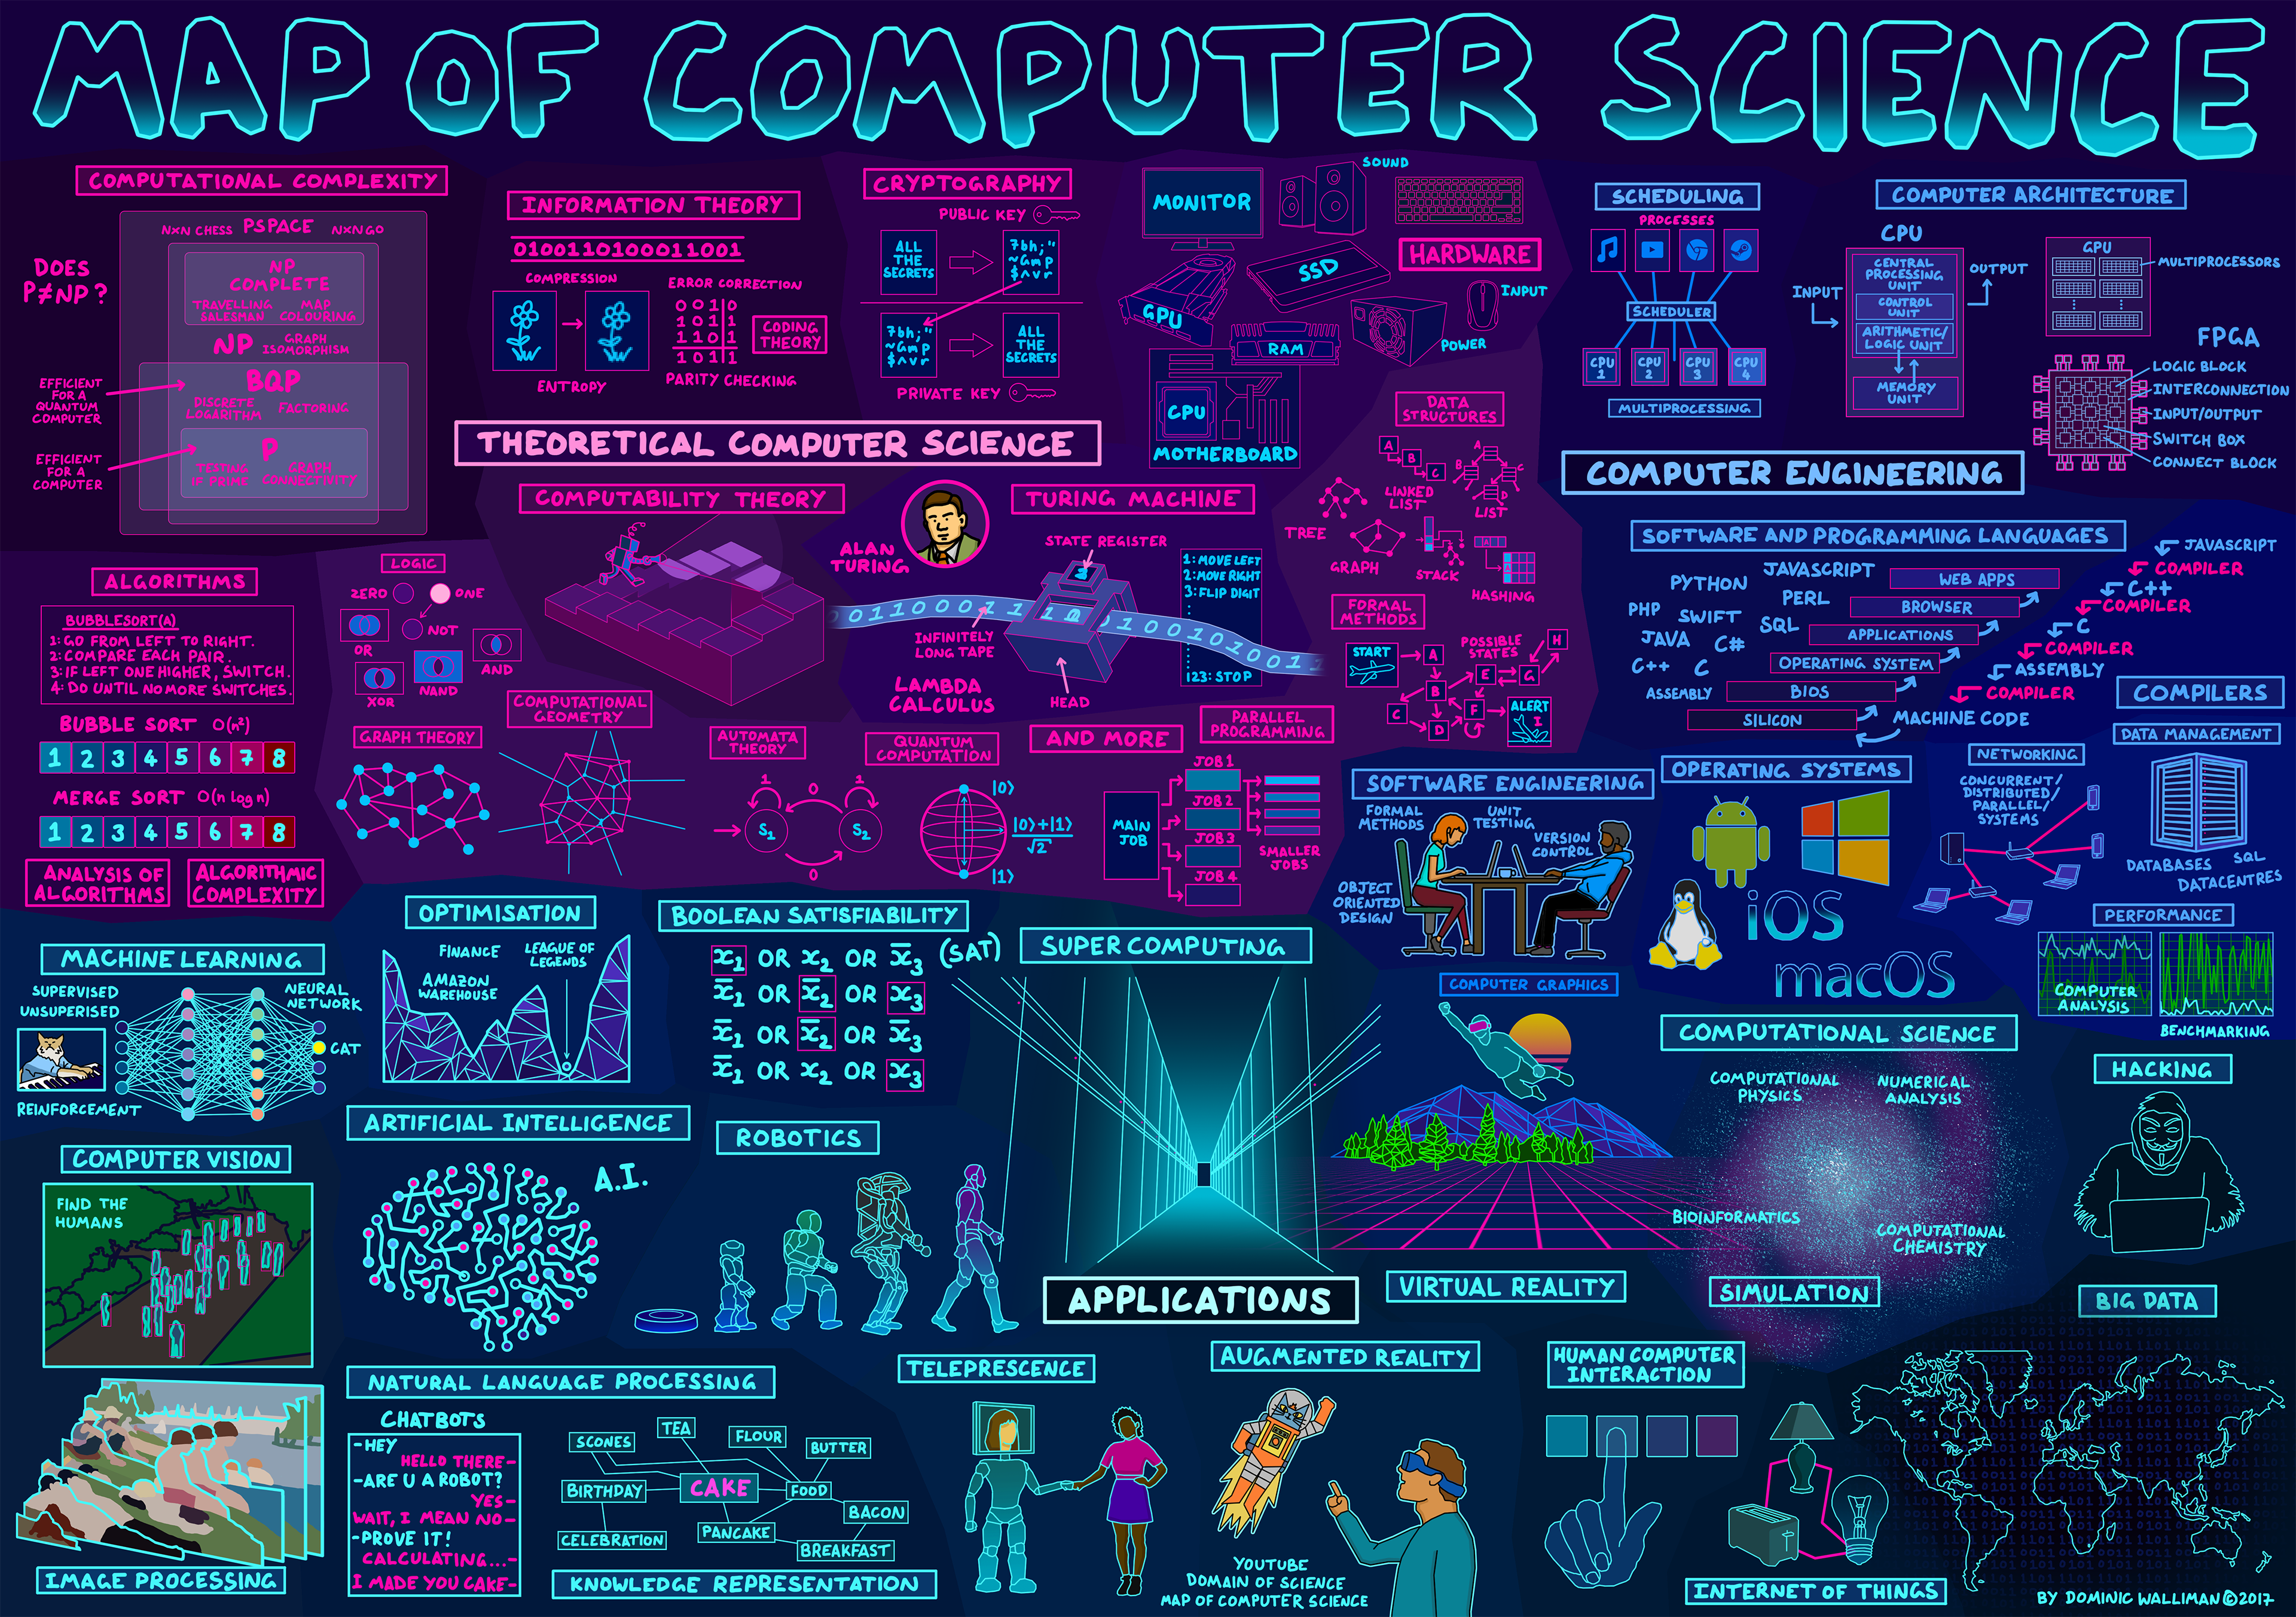
\includegraphics[width=\textwidth]{cs_map.png}
\end{frame}                                  

\begin{frame}{}

\end{document}
